%%---------------------------------------------------------------------------%%
%% mesh-type for imc-dev manual
%%---------------------------------------------------------------------------%%

\section{Mesh Types in \imctest}

\imctest\ is parameterized on the \comp{OS\_Mesh} (orthogonal-structured) 
class.  Ideally, any MT could be used in \imctest\ assuming it provided 
certain services.  Thus, extending \imctest\ to use AMR mesh-types only 
requires the construction of an \comp{AMR\_Mesh} class.  This
extensibility model is the motivating factor behind \draco\.

\subsection{\comp{OS\_Mesh} Class}

\subsubsection{Class Design}

The structure of the \comp{OS\_Mesh} class is illustrated in
Fig.~\ref{fig:os_mesh}.
\begin{figure}
\centerline{
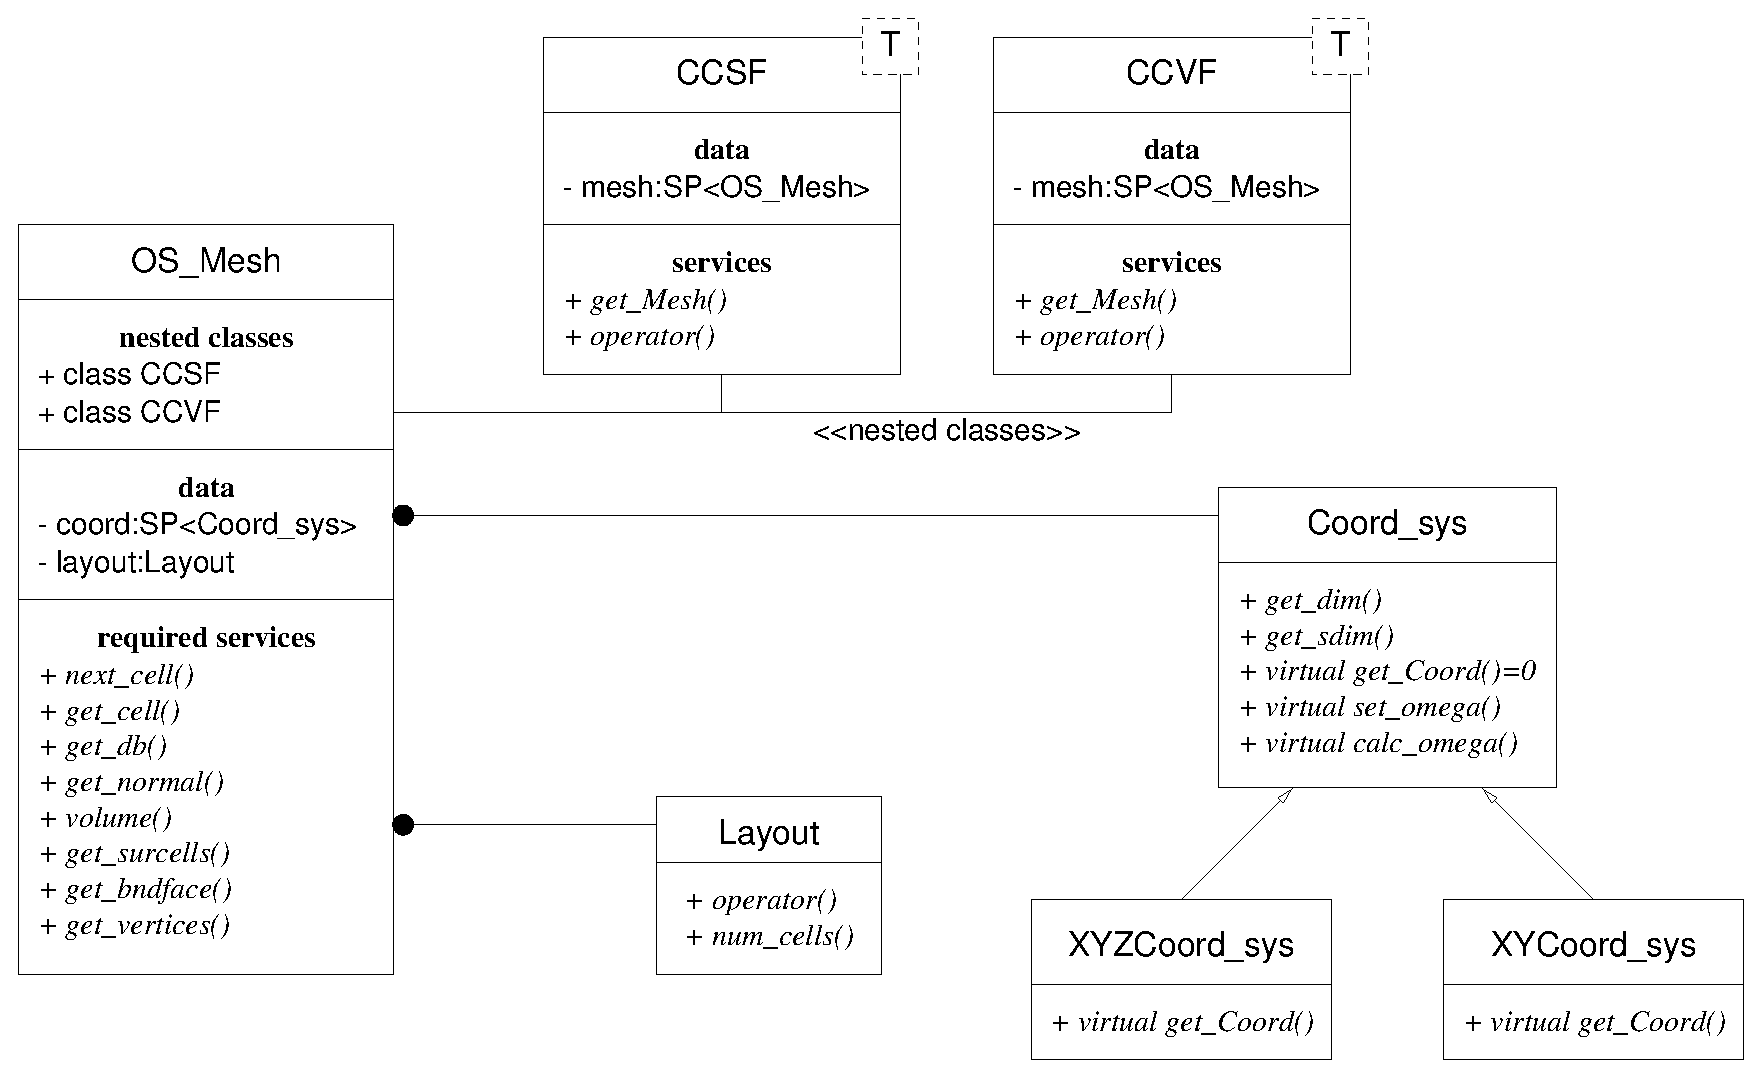
\includegraphics[width=5in]{os_mesh.eps}}
\caption{OS\_Mesh class design.}
\label{fig:os_mesh}
\end{figure}
\comp{OS\_Mesh} contains two nested service
classes which describe cell-centered quantities, \comp{CCSF}
(cell-centered scalar field) and \comp{CCVF} (cell-centered vector
field).  \comp{OS\_Mesh} also contains as data members two component
classes, \comp{Layout} and \comp{Coord\_sys}.  \comp{Layout} contains the
cell-face-cell information which is necessary for transporting
particles across a cell-face.  \comp{Coord\_sys} is a base class that
defines the coordinate system.  \comp{Coord\_sys} has two derived
classes, \comp{XYCoord\_sys} and \comp{XYZCoord\_sys}.  The derived
coordinate system classes define services necessary for transport
through a particular coordinate system.  The coordinate system member
in \comp{OS\_Mesh} is a base class smart pointer to one of these derived 
classes.

\subsubsection{\comp{OS\_Mesh} Interface}

The general public interface for \comp{OS\_Mesh} is displayed in
Fig.~\ref{os_mesh-int}.  \cdFramedFigure{os_mesh-int}{Public interface
  for the \comp{OS\_Mesh} class.}  To work successfully in the
\imctest\ package, a MT must provide several required services.  The
interface for these services are illustrated for the \comp{OS\_Mesh}
class in Fig.~\ref{os_mesh-rint}.
\cdFramedFigure{os_mesh-rint}{Required MT services for the
  \comp{OS\_Mesh} class.}

\subsection{\comp{Layout} Class}

The public interface for \comp{Layout} is shown in
Fig.~\ref{layout-int}.
\cdFramedFigure{layout-int}{Public interface for the \comp{Layout}
  class.}

\subsection{\comp{Coord\_sys} Class}

The public interface for the pure virtual base class \comp{Coord\_sys}
is shown in Fig.~\ref{coord_sys-int}.
\cdFramedFigure{coord_sys-int}{Public interface for the
  \comp{Coord\_sys} pure virtual base class.}

\subsubsection{\comp{Coord\_sys} Derived Classes.}

The public interfaces for the derived classes of \comp{Coord\_sys} are 
shown in Figs.~\ref{xycoord_sys-int} and \ref{xyzcoord_sys-int}.
\cdFramedFigure{xycoord_sys-int}{Public interface for the
  \comp{XYCoord\_sys} derived class.}
\cdFramedFigure{xyzcoord_sys-int}{Public interface for the
  \comp{XYZCoord\_sys} derived class.}
